
\documentclass[11pt]{article}

\usepackage[T1]{fontenc}
\usepackage[utf8]{inputenc}
\usepackage{mathptmx}
\usepackage[scaled]{helvet}

\usepackage[letterpaper,margin=1in]{geometry}
\usepackage{setspace}
\onehalfspacing

\usepackage{amsmath,amssymb,amsthm}
\usepackage{bm}
\usepackage{mathtools}

\usepackage{graphicx}
\usepackage{booktabs}
\usepackage{array}
\usepackage{tabularx}
\usepackage{longtable}
\usepackage[font=small,labelfont=bf]{caption}
\usepackage{float}

\usepackage{enumitem}
\usepackage{xcolor}
\usepackage[colorlinks=true,linkcolor=black,citecolor=black,urlcolor=blue]{hyperref}

\setlength{\emergencystretch}{2em}
\hfuzz=1pt
\newtheorem{theorem}{Theorem}[section]
\newtheorem{lemma}{Lemma}[section]
\newtheorem{proposition}{Proposition}[section]
\newtheorem{corollary}{Corollary}[section]
\theoremstyle{definition}
\newtheorem{definition}{Definition}[section]
\newtheorem{assumption}{Assumption}[section]
\theoremstyle{remark}
\newtheorem*{remark}{Remark}


\newcommand{\Tseed}{T_{\text{seed}}}
\newcommand{\Tint}{T_{\text{int}}}
\newcommand{\Pseed}{P_{\text{seed}}}
\newcommand{\Pint}{P_{\text{int}}}
\newcommand{\Epep}{E_{\text{PEP}}}
\newcommand{\Ebarpep}{\bar{E}_{\text{PEP}}}
\newcommand{\Faccess}{F_{\text{access}}}
\newcommand{\tcrit}{t_{\text{crit}}}
\newcommand{\emax}{\varepsilon_{\max}}
\newcommand{\emid}{\varepsilon_{\text{mid}}}
\newcommand{\emin}{\varepsilon_{\min}}

\setlength{\parskip}{0.4em}
\setlength{\parindent}{0pt}


\renewcommand{\thesection}{S\arabic{section}}
\renewcommand{\thesubsection}{S\arabic{section}.\arabic{subsection}}
\renewcommand{\thefigure}{S\arabic{figure}}
\renewcommand{\thetable}{S\arabic{table}}
\renewcommand{\theequation}{S\arabic{equation}}

\usepackage{titlesec}
\titleformat*{\section}{\large\bfseries}
\titleformat*{\subsection}{\normalsize\bfseries}


\bibliographystyle{plos2015}


\makeatletter
\renewcommand{\@biblabel}[1]{\quad#1.}
\makeatother


\begin{document}

\begin{flushleft}
{\Large\bfseries Supplementary Materials for\par}
\vspace{0.3em}
{\large\bfseries The HIV Post-Exposure Prophylaxis Window:
A Multiscale Framework Linking Within-Host Integration Kinetics to Population-Scale Structural Access\par}
\vspace{0.8em}
Adrian Charles (A.C) Demidont, DO\textsuperscript{*}\\
\textit{Nyx Dynamics LLC, Philadelphia, PA 19107, USA}\\
\textsuperscript{*}Correspondence: \texttt{acdemidont@nyxdynamics.com}\\
ORCID: 0000-0002-9216-8569
\end{flushleft}

\vspace{0.5em}
\hrule
\vspace{0.5em}

\noindent\textbf{This PDF file includes:}
\begin{itemize}[leftmargin=2em,nosep]
\item Sections S1--S6: Mathematical development with complete proofs
\item Section S7: Multiscale within-host model implementation
\item Section S8: NHP concordance --- per-timepoint detail
\item Section S9: Parameter tables
\item Section S10: Stochastic VL analysis --- extended methods
\item Section S11: City-stratified extended methods
\item Section S12: Figure inventory
\item Section S13: PK-driven PEP efficacy framework
\item Section S14: Pharmacy-access corridor and displacement analysis
\end{itemize}

\vspace{0.5em}



\section{Probability Space, State Definitions, and Assumptions}

Consider a single HIV exposure event $e$ occurring at time $t = 0$ on probability space $(\Omega, \mathcal{F}, \mathbb{P})$ with filtration $\{\mathcal{F}_{t}\}_{t \geq 0}$.

\subsection{Within-host states}

\begin{definition}[Within-host infection states]
$Z(t) \in \{0, 1, 2\}$:
\begin{itemize}[nosep,leftmargin=2em]
    \item $Z(t) = 0$ (Susceptible): no productive infection; $I(t) < I^{*}$.
    \item $Z(t) = 1$ (Seeded): replicative focus established ($I(t) \geq I^{*}$) but reservoir below irreversibility threshold ($R(t) < R^{*}$).
    \item $Z(t) = 2$ (Integrated): $R(t) \geq R^{*}$. Absorbing state under Assumption~A1.
\end{itemize}
\end{definition}

\begin{definition}[Transition stopping times]
\[
\Tseed = \inf\{t \geq 0 : Z(t) \geq 1\}, \qquad
\Tint  = \inf\{t \geq 0 : Z(t) = 2\}.
\]
We assume $\Tseed \leq \Tint$ almost surely.
\end{definition}

\begin{definition}[Cumulative transition probabilities]
$\Pseed(t) = \mathbb{P}(\Tseed \leq t)$, $\Pint(t) = \mathbb{P}(\Tint \leq t)$. Since $\Tseed \leq \Tint$ a.s., $\Pseed(t) \geq \Pint(t)$ for all $t \geq 0$.
\end{definition}

\subsection{Assumptions}

\begin{assumption}[Irreversibility of integration]
Once $Z(t) = 2$, the state is absorbing: $\mathbb{P}(Z(s) = 0 \mid Z(t) = 2) = 0$ for all $s > t$.

\textit{Biological grounding}: Integrated provirus persists for the lifetime of the host cell and propagates to daughter cells via clonal expansion. ART suppresses replication ($I \to 0$) but $dR/dt = \alpha I \to 0$: the reservoir is static under ART but does not shrink. No approved therapy achieves eradication.
\end{assumption}

\begin{assumption}[Stage-dependent drug efficacy]
\[
\varepsilon(Z(t)) =
\begin{cases}
\emax & Z(t) = 0,\\
\emid & Z(t) = 1,\\
\emin = 0 & Z(t) = 2,
\end{cases}
\qquad
\text{with } 1 \geq \emax \geq \emid \geq 0.
\]
\end{assumption}

\begin{assumption}[Monotonicity of integration]
$\Pint(t)$ is non-decreasing, $\Pint(0) = 0$, $\lim_{t\to\infty} \Pint(t) = 1$.
\end{assumption}

\begin{assumption}[Transmission-competent exposure]
Source plasma viral load is at or above the U=U threshold ($\geq 200$~copies/mL sustained). The framework is silent on exposures from virologically suppressed sources, for whom transmission risk is functionally zero (Rodger 2019, PARTNER2; Bavinton 2018, Opposites Attract).
\end{assumption}


\section{Master Equation}

\begin{proposition}[Master equation]\label{prop:master}
Under Assumption~A2,
\begin{equation}
\Epep(t) = \big(1 - \Pseed(t)\big)\emax + \big(\Pseed(t) - \Pint(t)\big)\emid + \Pint(t)\,\emin
\label{eq:master_si}
\end{equation}
\end{proposition}

\begin{proof}
Partition the sample space at time $t$ by $Z(t)$:
\[
\mathbb{P}(Z = 0) = 1 - \Pseed,\quad
\mathbb{P}(Z = 1) = \Pseed - \Pint,\quad
\mathbb{P}(Z = 2) = \Pint.
\]
These events are mutually exclusive and exhaustive. By the law of total expectation:
\[
\Epep(t) = \mathbb{E}[\varepsilon(Z(t))] = (1 - \Pseed)\,\emax + (\Pseed - \Pint)\,\emid + \Pint\,\emin. \qedhere
\]
\end{proof}


\section{The Finite Prevention Window Theorem}

\begin{theorem}[Finite Prevention Window]\label{thm:finite}
Under Assumptions~A1--A3, $\Epep(t)$ satisfies:
\begin{enumerate}[label=\textnormal{(\roman*)},leftmargin=2.5em]
    \item $\Epep(t) \leq \big(1 - \Pint(t)\big)\,\emax$;
    \item $\Epep(t)$ is non-increasing in $t$;
    \item $\Epep(t) \to 0$ as $t \to \infty$;
    \item for any $\eta \in (0,1)$, $\tcrit(\eta) = \inf\{t : \Epep(t) < \eta\}$ is finite.
\end{enumerate}
\end{theorem}

\begin{proof}
\textit{Part (i) --- Upper bound.} Replace $\emid$ with $\emax$ in (\ref{eq:master_si}):
\[
\Epep(t) \leq (1 - \Pseed)\emax + (\Pseed - \Pint)\emax + \Pint\,\emin = (1 - \Pint)\emax + \Pint\,\emin.
\]
With $\emin = 0$: $\Epep(t) \leq (1 - \Pint(t))\emax$.

\textit{Part (ii) --- Monotone decay.} For $t_{1} < t_{2}$, let $\Delta_{S} = \Pseed(t_{2}) - \Pseed(t_{1}) \geq 0$ and $\Delta_{I} = \Pint(t_{2}) - \Pint(t_{1}) \geq 0$. Then
\[
\Epep(t_{1}) - \Epep(t_{2}) = \Delta_{S}(\emax - \emid) + \Delta_{I}(\emid - \emin) \geq 0.
\]

\textit{Part (iii) --- Convergence.} By A3, $\Pint(t) \to 1$. Since $\Tseed \leq \Tint$ a.s., $\Pseed(t) \to 1$. Limits give $\Epep(t) \to 0\cdot\emax + 0\cdot\emid + 1\cdot\emin = 0$.

\textit{Part (iv) --- Finite critical time.} By (ii), $\Epep$ is non-increasing; by (iii), $\Epep \to 0 < \eta$. Therefore $\{t : \Epep(t) < \eta\}$ is non-empty, and $\tcrit(\eta)$ is finite.
\end{proof}


\section{Hazard-Rate Decomposition of Efficacy Loss}

\begin{definition}[Hazard rates]
$\lambda_{\text{seed}}(t) = f_{\text{seed}}(t)/(1 - \Pseed(t))$, $\lambda_{\text{int}}(t) = f_{\text{int}}(t)/(\Pseed(t) - \Pint(t))$.
\end{definition}

\begin{proposition}[Decomposition]\label{prop:hazard}
Under Assumptions~A1--A3 with absolute continuity,
\begin{equation}
\frac{d\Epep}{dt} = -f_{\text{seed}}(t)\,\Delta\varepsilon_{1} - f_{\text{int}}(t)\,\Delta\varepsilon_{2} \;\leq\; 0
\label{eq:hazard_si}
\end{equation}
where $\Delta\varepsilon_{1} = \emax - \emid$ and $\Delta\varepsilon_{2} = \emid - \emin$.
\end{proposition}

\begin{proof}
Differentiating (\ref{eq:master_si}):
\[
\frac{d\Epep}{dt} = -f_{\text{seed}}\emax + (f_{\text{seed}} - f_{\text{int}})\emid + f_{\text{int}}\emin = -f_{\text{seed}}\Delta\varepsilon_{1} - f_{\text{int}}\Delta\varepsilon_{2} \leq 0. \qedhere
\]
\end{proof}

\begin{remark}
Equation~\ref{eq:hazard_si} decomposes efficacy loss into a seeding channel ($f_{\text{seed}}$, gap $\Delta\varepsilon_{1}$) and an integration channel ($f_{\text{int}}$, gap $\Delta\varepsilon_{2}$). At early times, seeding dominates; as mass accumulates in state~1, the integration channel accelerates terminal efficacy collapse.
\end{remark}


\section{Route Compression and Inoculum-Monotone Hitting Times}

\subsection{ODE system}

The standard target-cell-limited within-host model:
\begin{equation}
\frac{dT}{dt} = \lambda - dT - \beta TV, \quad
\frac{dI}{dt} = \beta TV - \delta I, \quad
\frac{dV}{dt} = pI - cV, \quad
\frac{dR}{dt} = \alpha I
\label{eq:ode}
\end{equation}
where $T$ = target cells, $I$ = infected cells, $V$ = free virions, $R$ = cells with stable proviral integration.

\begin{lemma}[Absorbing state]\label{lem:absorb}
The set $\mathcal{A} = \{R > 0\}$ is positively invariant. If $R(t_{0}) > 0$ then $R(t) > 0$ for all $t > t_{0}$.
\end{lemma}

\begin{proof}
$dR/dt = \alpha I \geq 0$, so $R$ is non-decreasing. Under ART, $I \to 0$ and $dR/dt \to 0$: the reservoir is static but does not shrink.
\end{proof}

\subsection{Route-dependent initial conditions}

$V^{(m)}(0) = 1$ virion/mL (mucosal, post-epithelial attenuation) versus $V^{(p)}(0) = 10^{3}$ virions/mL (parenteral, direct intravascular delivery). All ODE parameters in (\ref{eq:ode}) are identical across routes.

\begin{lemma}[Inoculum-monotone hitting times]\label{lem:monotone}
Solutions of (\ref{eq:ode}) with $V(0) = v_{0} < \tilde{V}(0) = \tilde{v}$ satisfy $\tilde{I}(t) \geq I(t)$ and $\tilde{R}(t) \geq R(t)$ for all $t \geq 0$. Therefore $\Tint(\tilde{v}) \leq \Tint(v_{0})$ a.s.
\end{lemma}

\begin{proof}
The subsystem $(I, V, R)$ is cooperative for fixed $T$:
\[
\frac{\partial(\beta TV)}{\partial V} \geq 0, \quad
\frac{\partial(pI)}{\partial I} \geq 0, \quad
\frac{\partial(\alpha I)}{\partial R} = 0.
\]
By comparison theorems for cooperative ODE systems\cite{smith1995}, solutions are order-preserving in initial conditions. Since $\tilde{V}(0) > V(0)$: $\tilde{V}(t) \geq V(t)$ and $\tilde{I}(t) \geq I(t)$ for all $t \geq 0$. Then
\[
\tilde{R}(t) = \alpha \int_{0}^{t} \tilde{I}(s)\,ds \;\geq\; \alpha \int_{0}^{t} I(s)\,ds = R(t),
\]
so $\Tint(\tilde{v}) \leq \Tint(v_{0})$.
\end{proof}

\subsection{Route compression corollary}

\begin{assumption}[Stochastic dominance]
$\Pint^{(p)}(t) \geq \Pint^{(m)}(t)$ for all $t \geq 0$. Follows from Lemma~\ref{lem:monotone} under route-specific inocula.
\end{assumption}

\begin{corollary}[Route compression]\label{cor:route}
Under Assumptions~A1--A4:
\begin{enumerate}[label=\textnormal{(\roman*)},leftmargin=2.5em]
    \item $\Epep^{(p)}(t) \leq \Epep^{(m)}(t)$;
    \item $\tcrit^{(p)}(\eta) \leq \tcrit^{(m)}(\eta)$.
\end{enumerate}
\end{corollary}

\begin{proof}
(i) The weight on $\emax$ equals $1 - \Pseed(t)$, which is smaller for parenteral; the weight on $\emin = 0$ equals $\Pint(t)$, which is larger for parenteral. So $\Epep^{(p)} \leq \Epep^{(m)}$.

(ii) Both functions are non-increasing; $\tcrit^{(p)}(\eta) = \inf\{t : \Epep^{(p)} < \eta\} \leq \inf\{t : \Epep^{(m)} < \eta\} = \tcrit^{(m)}(\eta)$.
\end{proof}


\section{Analytical Population-Level Consistency Bound}
\begin{definition}
$\Ebarpep = \mathbb{E}[\Epep(T_{\text{access}})] = \int_{0}^{\infty} \Epep(t)\,d\Faccess(t)$.
\end{definition}

\begin{proposition}[Conservative timing consistency bound]\label{prop:bound}
Under Assumptions~A1--A4,
\begin{equation}
\Ebarpep \;\leq\; \Faccess(\tcrit)\,\emax + \big(1 - \Faccess(\tcrit)\big)\,\eta
\label{eq:bound_si}
\end{equation}
\end{proposition}

\begin{proof}
Partition the integral at $\tcrit(\eta)$:
\[
\Ebarpep = \int_{0}^{\tcrit} \Epep(t)\,d\Faccess + \int_{\tcrit}^{\infty} \Epep(t)\,d\Faccess
\;\leq\; \emax\,\Faccess(\tcrit) + \eta\,(1 - \Faccess(\tcrit)),
\]
using $\Epep(t) \leq \emax$ for $t \leq \tcrit$ and $\Epep(t) < \eta$ for $t > \tcrit$ (Theorem~\ref{thm:finite}(iv)).
\end{proof}

\subsection{Worked example (verified numerical values)}

Using the multiscale model output at the canonical operating point ($V_{0} = 10^{3}$ parenteral, CV $= 0.3$ on $\beta, c, \delta, \alpha$; commit \texttt{37e27ea}), $\tcrit^{(p)}(0.05) \approx 34.5$~h. Modeling access delay as log-normal (median 96~h, geometric SD 2.0):
\[
\Faccess(34.5~\text{h}) = \Phi\!\left(\frac{\ln 34.5 - \ln 96}{\ln 2}\right) = \Phi(-1.476) \approx 0.0699.
\]
With $\eta = 0.05$ and $\emax = 0.95$:
\[
\Ebarpep \;\leq\; 0.0699 \times 0.95 + 0.9301 \times 0.05 \;\approx\; 0.113.
\]
Envelope reading: expected population PEP efficacy below approximately 11.3\%.

\subsection{Sensitivity of the envelope to \texorpdfstring{$\Faccess$}{Faccess} parameterization}

The median time-to-PEP-access for PWID is not directly anchored by primary timing data in the cited references (Taylor 2019\cite{taylor2019_si} is a 3-page commentary; Baugher 2025\cite{baugher2025_si} is NHBS-PWID surveillance focused on PrEP/syringe metrics, not PEP timing). The median is therefore a modeling choice informed by qualitative discussion of structural barriers in those references. Sensitivity:

\begin{table}[H]
\centering
\small
\caption{Envelope sensitivity to $\Faccess$ median (GSD $= 2.0$, $\tcrit^{(p)} = 34.5$~h, $\eta = 0.05$, $\emax = 0.95$).}
\begin{tabular}{@{}lcc@{}}
\toprule
\textbf{Median} & \textbf{$\Faccess(34.5\,\text{h})$} & \textbf{Envelope $\Ebarpep$} \\
\midrule
72~h (JID-consistent) & 0.144 & $\leq 18.0\%$ \\
96~h (canonical)      & 0.070 & $\leq 11.3\%$ \\
110~h                 & 0.047 & $\leq 9.2\%$  \\
120~h                 & 0.036 & $\leq 8.2\%$  \\
\bottomrule
\end{tabular}
\end{table}

This inequality is retained as a conservative analytical ceiling and consistency check on the timing argument. It is not a full population preventability estimator because it collapses access into $\Faccess(\tcrit)$ and does not model the per-patient PK/PD corridor introduced in Section~\ref{sec:S2_corridor}. In independent cascade-based modeling of structural access (companion analysis; see main text Population-level implications section), point estimates of $P(R_{0}=0)$ for PWID under current US policy are 0.003--0.7\%, one to four orders of magnitude below this ceiling. Thus the bound provides a least-pessimistic analytical check, while the cascade model provides central estimates and the corridor analysis provides the mechanistic access interpretation.

\subsection{Limitation: \texorpdfstring{$\Faccess$}{Faccess} denominator}

$\Faccess$ derives from population-wide PEP-access surveillance, which includes exposures from both transmission-competent and virologically suppressed sources. Under U=U (Assumption~A4), exposures from suppressed sources are outside the framework's domain. Restricting $\Faccess$ to transmission-competent exposures only would reduce the relevant denominator and yield a tighter (smaller) $\Faccess$ and therefore a tighter envelope. The reported envelope is thus conservative with respect to U=U scoping: the true within-domain envelope is no larger than the reported value.


\section{Multiscale Within-Host Model: Implementation}

The multiscale within-host model combines stochastic founder-phase dynamics with deterministic ODE integration once productive infection is established. This section documents the implementation; all code is reproducible from \texttt{SRC/multiscale\_model/} at commit \texttt{37e27ea} of the project repository.

\subsection{Phase~1: Stochastic founder-phase tau-leaping}

At low founder population ($V_{0} \leq I_{\text{handoff}} = 10$), the dynamics are sensitive to extinction events; deterministic integration of (\ref{eq:ode}) systematically underestimates the extinction probability and overestimates the rate of reservoir establishment. Phase~1 uses tau-leaping integration of the discrete-state Markov chain with reactions:
\[
T \xrightarrow{\beta T V} I, \qquad I \xrightarrow{\delta} \emptyset, \qquad I \xrightarrow{p} I + V, \qquad V \xrightarrow{c} \emptyset, \qquad I \xrightarrow{\alpha} R.
\]
A fixed-delay buffer of $\tau_{\text{eclipse}} = 0.9$ days ($\approx 22$~h, Perelson 1996 Table~2)\cite{perelson1996_si} is enforced between cell infection and integration competence, ensuring that the lower bound on $\Tint$ matches the biological eclipse floor regardless of population dynamics.

A realization is classified as \emph{extinct} if both $I(t)$ and $V(t)$ reach zero before the population threshold $I_{\text{handoff}} = 10$ is exceeded. A realization is classified as \emph{integrated} if $R(t) \geq R^{*} = 10$ cells/mL is reached. For mucosal exposure ($V_{0} = 1$), extinction probability under CV $= 0.3$ is $\approx 68\%$; for parenteral exposure ($V_{0} = 10^{3}$, CV $= 0.3$), extinction is essentially zero ($<0.5\%$).

\subsection{Phase~2: Deterministic ODE handoff}

Once $I(t)$ exceeds $I_{\text{handoff}} = 10$, the dynamics transition to deterministic integration of (\ref{eq:ode}) using \texttt{scipy.integrate.solve\_ivp} with adaptive step size. The handoff continues until $R(t) \geq R^{*}$, at which point $\Tint$ is recorded.

\subsection{Heterogeneity}

Inter-individual variability is modeled as multiplicative log-normal noise on $\{\beta, c, \delta, \alpha\}$ with coefficient of variation $0.3$. The noise parameters are sampled once per realization; deterministic phase parameters use the sampled values throughout. The CV $= 0.3$ value is consistent with the standard within-host model heterogeneity assumption used in earlier published noise-anchored models.

\subsection{Sample size and seeding}

We use $N = 500$ realizations per (route, $V_{0}$, CV) cell. Random seeds are deterministic: \texttt{rng = np.random.default\_rng(base\_seed*1{,}000{,}000+k)} where $k$ is the realization index. This guarantees byte-identical reproducibility from a cloned repository at the cited SHA. Sensitivity to $N$ at the canonical operating point is reported in main text Methods; $\tcrit$ estimates are stable to $\pm 0.5$~h across $N \in \{200, 500, 1000, 5000\}$.

\subsection{Output: \texorpdfstring{$\tcrit$}{tcrit} and \texorpdfstring{$\Pint(t)$}{Pint(t)}}

For each cell, the empirical CDF $\Pint(t)$ is constructed from the $N$-realization integration-time distribution. The route-specific efficacy curve $\Epep(t)$ is computed from $\Pint(t)$ via the master equation (\ref{eq:master_si}), and $\tcrit(\eta)$ is the smallest $t$ at which $\Epep(t) < \eta$. Reported $\tcrit$ values:

\begin{table}[H]
\centering
\small
\caption{Verified $\tcrit$ at $\eta = 0.05$ from \texttt{SRC/multiscale\_model/results\_v3/heterogeneity\_summary.csv}.}
\begin{tabular}{@{}llcc@{}}
\toprule
\textbf{Route} & \textbf{$V_{0}$} & \textbf{CV} & \textbf{$\tcrit(0.05)$ [h]} \\
\midrule
Parenteral  & $10^{3}$ & 0.0 & 32.5 \\
Parenteral  & $10^{3}$ & 0.3 & \textbf{34.5} \\
Parenteral  & $10^{3}$ & 0.5 & 36.0 \\
Mucosal     & 1        & 0.0 & 57.5 \\
Mucosal     & 1        & 0.3 & \textbf{60.5} \\
Mucosal     & 1        & 0.5 & 60.0 \\
\bottomrule
\end{tabular}
\end{table}

The compression ratio at the canonical operating point (CV $= 0.3$) is $60.5/34.5 \approx 1.75\times$.


\section{NHP Concordance --- Per-Timepoint Detail}

The multiscale model output was compared to NHP empirical protection rates at the timepoints reported in Tsai 1998\cite{tsai1995_si} and Otten 2000\cite{otten2000_si}. Concordance is defined as $|\Epep(\text{delay}) - \text{NHP protection}| < 0.20$ (within 20 percentage points).

\begin{table}[H]
\centering
\small
\caption{Per-timepoint NHP concordance at the canonical operating point (CV $= 0.3$). Reproducible from \texttt{SRC/multiscale\_model/results\_v3/nhp\_concordance.csv}.}
\begin{tabular}{@{}llccccc@{}}
\toprule
\textbf{Study} & \textbf{Route} & \textbf{Delay [h]} & \textbf{NHP protection} & \textbf{Model $\Epep$} & \textbf{$|$diff$|$ [pp]} & \textbf{Concordant} \\
\midrule
Otten 2000      & mucosal    & 12 & 1.00 & 0.95 & 5.0  & yes \\
Otten 2000      & mucosal    & 36 & 1.00 & 0.95 & 5.0  & yes \\
Otten 2000      & mucosal    & 72 & 0.50 & 0.016 & 48.4 & no  \\
Tsai 1998 IV    & parenteral & 24 & 1.00 & 0.50 & 50.0 & no  \\
Tsai 1998 IV    & parenteral & 48 & 0.50 & 0.00 & 50.0 & no  \\
\bottomrule
\end{tabular}
\end{table}

\textbf{Compression-ratio concordance.} The model's mucosal/parenteral $\tcrit$ ratio at $\eta = 0.05$ is $60.5/34.5 \approx 1.75\times$. The empirical NHP compression ratio between Tsai 1998 IV (parenteral half-protection at 48~h) and Otten 2000 (mucosal half-protection at 72~h) is $72/48 = 1.50\times$. The model's compression value is concordant with the empirical NHP range of 1.5--2$\times$.

\textbf{Per-timepoint absolute discordance.} The within-host kinetic model under-predicts protection at:
\begin{itemize}[nosep,leftmargin=2em]
    \item Tsai 1998 IV at 24~h (model 0.50 vs.\ NHP 1.00),
    \item Tsai 1998 IV at 48~h (model 0.00 vs.\ NHP 0.50),
    \item Otten 2000 at 72~h (model 0.016 vs.\ NHP 0.50).
\end{itemize}
We interpret this gap as evidence of NHP-specific protective contributions not captured by the within-host kinetic framework alone. Possible mechanisms include innate immunity contributions during the eclipse phase, mucosal containment by epithelial defense, and the small NHP cohort size ($n = 2$--4 per group) producing wider empirical confidence intervals on observed protection rates than the model's first-passage formulation accommodates. The compression-ratio result and the absolute-timepoint result are independent: the compression result is robust to the model's domain limitations; absolute-timepoint discordance constrains the interpretation of the model as a kinetic-only ceiling rather than a full mechanistic prediction of NHP protection.


\section{Parameter Tables}

\subsection{ODE system parameters (Perelson 1996 anchored)}

\begin{table}[H]
\centering
\small
\caption{ODE system parameters anchored on Perelson et al.\ 1996 (PMID 8599114).}
\begin{tabular}{@{}llllp{4.5cm}@{}}
\toprule
\textbf{Symbol} & \textbf{Description} & \textbf{Value} & \textbf{Units} & \textbf{Source} \\
\midrule
$\delta$ & Infected cell death rate & 0.7 & day$^{-1}$ ($t_{1/2} \approx 1.6$d) & Perelson 1996, Table~1 \\
$c$ & Viral clearance rate & 23 & day$^{-1}$ ($t_{1/2} = 0.24$d $\approx 6$h) & Perelson 1996, Table~1 \\
$\tau$ & Viral generation time & 2.6 & days ($\approx 62$h) & Perelson 1996, Table~2 \\
Eclipse phase & Min time to integration competence & 0.9 & days ($\approx 22$h) & Perelson 1996, Table~2 \\
$\beta$ & Infection rate constant & $2.4 \times 10^{-5}$ & mL$\cdot$virion$^{-1}\cdot$day$^{-1}$ & Standard model \\
$p$ & Virion production per infected cell & $10^{3}$ & virions/cell/day & Standard model \\
$\alpha$ & Stable integration rate & $10^{-3}$ & day$^{-1}$ & Calibrated \\
\bottomrule
\end{tabular}
\end{table}

Parameters $c$ and $\delta$ directly from Table~1; eclipse phase and generation time from Table~2. \textit{Note:} the reference $\log_{10}$ VL $= 4.5$ for PWID is from NHBS/NHAS surveillance, not from Perelson 1996 (whose patients had mean $\log_{10}$ VL $\approx 5.3$).

\subsection{Drug efficacy parameters}

\begin{table}[H]
\centering
\small
\caption{Stage-dependent drug efficacy parameters.}
\begin{tabular}{@{}llcp{6.5cm}@{}}
\toprule
\textbf{Parameter} & \textbf{Value} & \textbf{State $Z(t)$} & \textbf{Justification} \\
\midrule
$\emax$ (pre-seeding) & 0.95 & $Z(t) = 0$ & Near-complete suppression of initial RT; consistent with tenofovir/FTC NHP protection data \\
$\emid$ (seeded/pre-int) & 0.50 & $Z(t) = 1$ & Partial suppression of established replicative focus; sensitivity $\pm 40\%$ shifts $\tcrit < 6$h \\
$\emin$ (integrated) & 0 (fixed) & $Z(t) = 2$ & ART does not eradicate provirus; set to 0 by A2 and Lemma~\ref{lem:absorb} \\
\bottomrule
\end{tabular}
\end{table}

\subsection{Route-specific initial conditions and thresholds}

\begin{table}[H]
\centering
\small
\caption{Route-specific initial conditions and threshold parameters.}
\begin{tabular}{@{}lllp{6cm}@{}}
\toprule
\textbf{Parameter} & \textbf{Mucosal} & \textbf{Parenteral} & \textbf{Note} \\
\midrule
$V(0)$ virions/mL & 1 & $10^{3}$ & 3-log difference drives route compression; post-epithelial attenuation vs.\ direct IV delivery \\
$T(0)$ CD4 cells/mL & $10^{6}$ & $10^{6}$ & Identical; peripheral blood \\
$I(0)$ and $R(0)$ & 0 & 0 & No infected cells or reservoir at exposure \\
$I^{*}$ (seeding threshold) & 100 cells/mL & 100 cells/mL & Sensitivity: $[10, 1000]$; $\tcrit$ shifts $<8$h; compression ratio stable \\
$R^{*}$ (integration threshold) & 10 cells/mL & 10 cells/mL & Sensitivity: $[1, 100]$; parenteral/mucosal ratio stable 1.5--2$\times$ \\
$I_{\text{handoff}}$ (Phase 1$\to$2) & 10 cells/mL & 10 cells/mL & Stochastic-to-deterministic transition threshold \\
\bottomrule
\end{tabular}
\end{table}

\subsection{Multiscale simulation parameters}

\begin{table}[H]
\centering
\small
\caption{Multiscale simulation parameters.}
\begin{tabular}{@{}lll@{}}
\toprule
\textbf{Parameter} & \textbf{Value} & \textbf{Description} \\
\midrule
$N$ Monte Carlo replications & 500 / cell & Per (route, $V_{0}$, CV) cell; total $\sim$27{,}000 across full sweep \\
Heterogeneity CV & 0.3 & Multiplicative log-normal on $\{\beta, c, \delta, \alpha\}$ \\
Random seed & deterministic & \texttt{rng = np.random.default\_rng(42*1{,}000{,}000+k)} \\
Tau-leaping step & adaptive & Phase 1, founder-phase \\
ODE integrator & \texttt{solve\_ivp} (LSODA) & Phase 2, deterministic handoff \\
Eclipse delay buffer & 0.9 days ($\approx 22$h) & Fixed delay between cell infection and integration competence \\
CI type & 95\% credible interval & From stochastic $\Tint$ distribution \\
\bottomrule
\end{tabular}
\end{table}


\section{Stochastic VL Analysis --- Extended Methods}

\subsection{Source VL distributions}

Expected PEP efficacy was computed as a Monte Carlo integral over source viral load:
\begin{equation}
\mathbb{E}[\Epep(t)] = \int \Epep(t, \text{VL})\,P(\text{VL})\,d\text{VL}
\label{eq:mc_integral}
\end{equation}

\begin{table}[H]
\centering
\small
\caption{Source VL distributions parameterized from surveillance data. All log10-normal.}
\begin{tabular}{@{}llcp{6cm}@{}}
\toprule
\textbf{Distribution} & \textbf{Mean $\log_{10}$} & \textbf{SD} & \textbf{Empirical basis} \\
\midrule
PWID untreated/unsuppressed & 4.5 & 1.1 & NHBS/NHAS surveillance; chronic untreated HIV-1 in PWID networks \\
PWID mixed treatment & 3.2 & 1.5 & Mixture: suppressed ($\sim 1.5$) + unsuppressed ($\sim 4.5$) in partially treated PWID networks \\
General HIV+ community & 3.8 & 1.2 & Mixed treatment uptake; heterogeneous MSM/general community networks \\
Acute-infection-enriched & 5.0 & 0.9 & High-transmission networks; acute viremia peak; recent-infection clustering \\
\bottomrule
\end{tabular}
\end{table}

\textit{Note:} PWID untreated mean $\log_{10} = 4.5$ is from NHBS/NHAS surveillance, NOT from Perelson 1996.

\subsection{Three-regime temporal classification}

\begin{table}[H]
\centering
\small
\caption{Three-regime CI-width classification for the PWID untreated distribution.}
\begin{tabular}{@{}lp{4cm}lp{5cm}@{}}
\toprule
\textbf{Regime} & \textbf{Hours (PWID untreat.)} & \textbf{Peak CI width} & \textbf{Clinical interpretation} \\
\midrule
1 --- Early window & 0--22.0~h & $<$15~pp & VL uncertainty low-impact; initiate PEP immediately regardless of source VL \\
2 --- Critical window & 22.0--78.4~h (PWID/acute); 22.0--88.2~h (mixed/general) & 39.7~pp at 49~h & Maximal VL uncertainty; source VL testing clinically actionable; VL premium peaks at 21~h \\
3 --- Late window & 78.4--120~h (PWID/acute); 88.2--120~h (mixed/general) & $<$10~pp (collapsed) & Efficacy uniformly poor; VL irrelevant; $P$(futile) $> 90\%$ \\
\bottomrule
\end{tabular}
\end{table}

The Regime 1/2 boundary at 22.04~h is consistent across all four VL distributions (eclipse phase lower bound, Perelson 1996). The Regime 2/3 boundary is distribution-dependent: 78.37~h for PWID untreated and acute-infection-enriched distributions (higher VL accelerates CI collapse); 88.16~h for mixed-treatment and general-community distributions. This distribution-specificity is biologically coherent: higher inoculum populations exhaust the critical window earlier.

\subsection{VL knowledge premium and non-monotonic plateau}

VL knowledge premium $=$ absolute difference in expected $\Epep(t)$ between known vs.\ unknown source VL. Peak values: 3.76~pp at 21~h (acute-enriched); 2.94~pp (PWID untreated); 1.87~pp (general community); 1.27~pp (mixed Tx). All distributions peak at 21~h --- maximal VL-knowledge value at critical window onset.


\section{City-Stratified Analysis --- Extended Methods}

\subsection{Data source}

City-level HIV surveillance data were extracted from AIDSVu downloadable datasets for 34 high-burden US metropolitan areas (2023 reporting year; downloaded October 2025).

\subsection{Mixture-model VL derivation}

\begin{equation}
\mu_{\text{mix}} = f_{s}\,\mu_{\text{suppressed}} + (1 - f_{s})\,\mu_{\text{unsuppressed}}
\label{eq:mixture}
\end{equation}

Suppressed: $\log_{10}$ mean $= 1.5$, SD $= 0.4$. Unsuppressed: $\log_{10}$ mean $= 4.5$, SD $= 1.1$. IDU correction: $f_{s}$ reduced by 0.12~percentage points per percent IDU prevalence, capped at 12~percentage points total.

\subsection{Structural delay: composite indicator (not proxy)}

\begin{equation}
\Delta t_{\text{structural}} = \beta_{1}\,(\text{LateDx}\% - 10\%) + \beta_{2}\,\max(90\% - \text{Linkage}\%,\,0) + \Delta t_{\text{SDOH}}
\label{eq:delay_si}
\end{equation}

$\beta_{1} = 1.2$~h/\%; $\beta_{2} = 0.3$~h/\%. SDOH modifier 0--6~h from Gini + poverty. Barrier categories: low ($<$8~h), moderate (8--18~h), high (18--30~h), severe ($\geq$30~h).

\textbf{Methodological note.} City-level structural delay $\Delta t_{\text{structural}}$ is a composite indicator constructed as a calibrated linear function of two AIDSVu surveillance variables (late-diagnosis percentage; linkage-to-care percentage) plus an SDOH modifier. The composite is not a proxy for an unmeasured latent construct under proximal causal inference\cite{tchetgentchetgen2020_si}, and the analysis does not invoke the identification conditions required for proxy-based estimation\cite{pearl2009_si}. Coefficients $\beta_{1}, \beta_{2}$ are calibrated to reproduce the median city-level access friction; the composite is interpreted as a description of healthcare access friction at the city level,  not as an estimator for a separate latent variable.

\subsection{Counterfactual analysis}

Parallel simulation assigning all 34 cities a uniform 24-hour access delay isolates structural barrier contribution from community VL. 33/34 cities show observed efficacy $>$ counterfactual (structural delays $<$24~h). Hartford CT is the sole exception (delay 24.4~h; high-barrier category, 18--30~h). Counterfactual range across cities: 76.0\%--82.1\%.


\section{Figure Inventory}

\subsection{Figure S1 --- Focused City Comparison}

\begin{figure}[H]
\centering
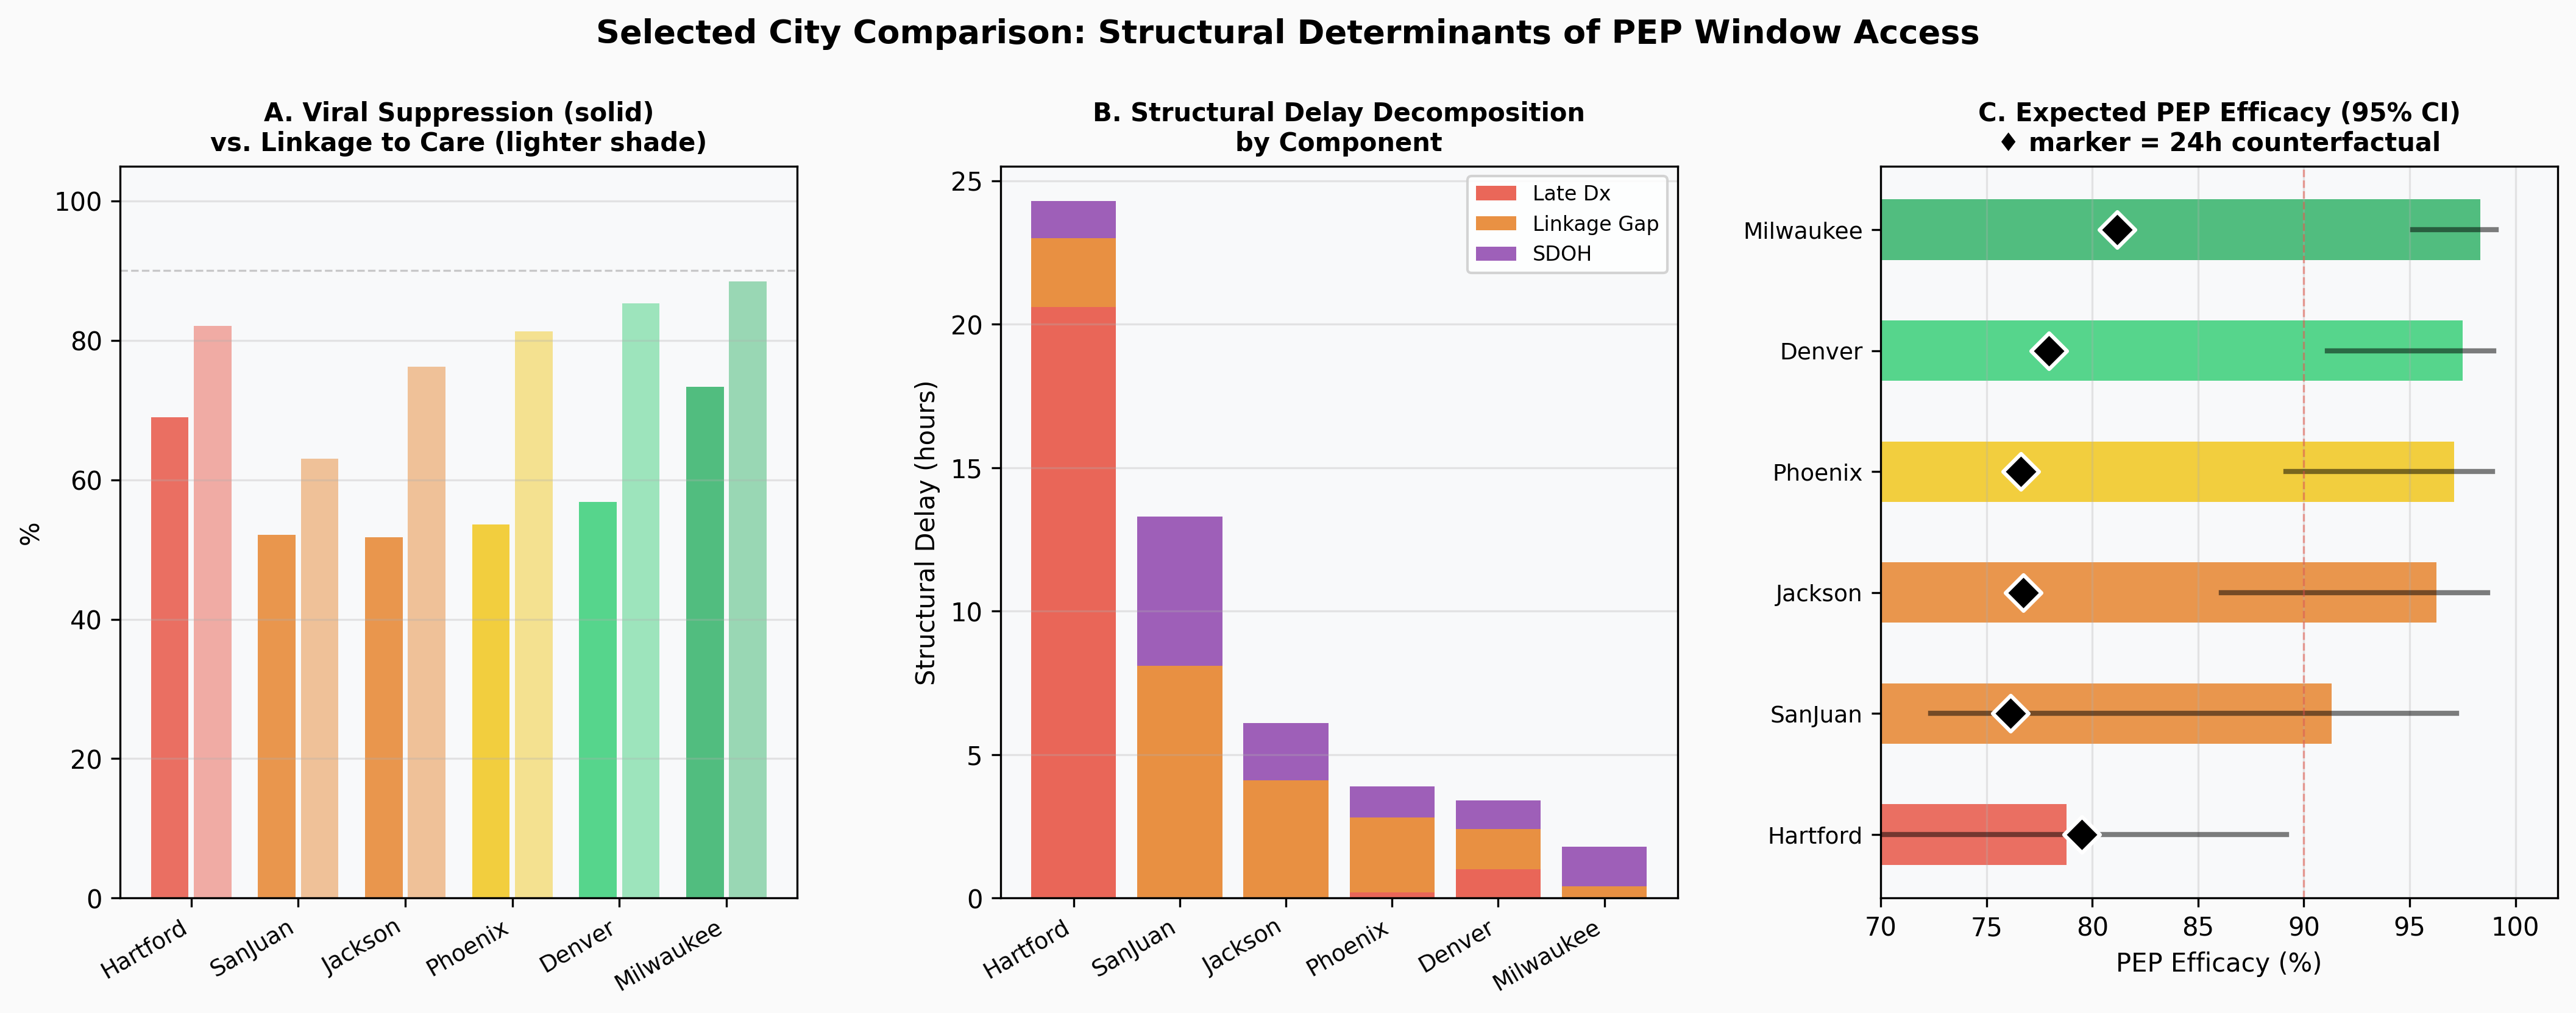
\includegraphics[width=\textwidth]{Figure_S1_CityComparison_Focus.png}
\caption{\textbf{Supplementary Figure S1. Selected city comparison: structural determinants of PEP window access.} Six high-vulnerability US cities (Hartford CT, San Juan PR, Jackson MS, Phoenix AZ, Denver CO, Milwaukee WI), ranked left-to-right from highest to lowest structural barrier.
(\textbf{A}) Viral suppression rate (solid bars) vs.\ linkage-to-care rate (lighter shade), per AIDSVu 2023.
(\textbf{B}) Structural-delay decomposition by component: late-diagnosis ($\beta_{1}$ contribution), linkage gap ($\beta_{2}$ contribution), and SDOH modifier. Hartford's 24.4-hour structural delay decomposes as Late Dx $\approx 21$~h, Linkage Gap $\approx 3$~h, SDOH $\approx 3$~h, identifying late-diagnosis as the dominant driver.
(\textbf{C}) Expected PEP efficacy at city-specific structural delay (95\% credible-interval bars; $\diamond$ marker $=$ 24-hour counterfactual). Hartford is the only city among the 34 in Figure~3 where actual expected efficacy falls below the 24-hour counterfactual, reflecting structural-delay overshoot.}
\label{fig:S1_focus}
\end{figure}
\newpage
  


\section{PK-Driven PEP Efficacy: Kinetic Onset Framework Implementation}
\label{sec:S10}

This section documents the implementation of the PK-driven framework, which generalizes the hand-set stage efficacies ($\emax = 0.95$, $\emid = 0.50$, $\emin = 0$) of the baseline formulation into a kinetic-onset formulation derived from drug pharmacokinetics, pharmacodynamics, and stage biology.

\subsection{Overview and decomposition}

For PEP initiation at time $t_{\text{PEP}}$ post-exposure, the stage-dependent drug efficacy is
\[
\varepsilon(Z, t_{\text{PEP}}) = \varepsilon_{\text{drug}}(t_{\text{PEP}}) \cdot p_{\text{clear}}(Z),
\]
where $\varepsilon_{\text{drug}}$ is purely pharmacologic and $p_{\text{clear}}$ is purely biological. The two quantities are separately identifiable and separately parameterizable.

\subsection{Pharmacokinetic model}

The PEP regimen is TDF/FTC + DTG per CDC 2025 recommendations\cite{tanner2025_si}. Drug-level kinetics use a one-compartment Bateman model with first-order absorption:
\[
C_{\text{plasma}}(t) = \frac{F \cdot D \cdot k_a}{V_d \cdot (k_a - k_e)} \left( e^{-k_e t} - e^{-k_a t} \right),
\]
where $F$ is bioavailability, $D$ dose, $k_a$ absorption rate, $k_e$ elimination rate, and $V_d$ volume of distribution. For the two NRTIs, the pharmacologically active species is the intracellular phosphorylated metabolite (TFV-DP for tenofovir; FTC-TP for emtricitabine); intracellular concentrations follow a downstream compartment driven by $C_{\text{plasma}}$ with formation rate $k_{\text{form}}$ and intracellular elimination rate $k_{e,\text{IC}}$. For DTG, the plasma compartment is itself active. Volumes of distribution were calibrated to reproduce literature steady-state AUC$_{24}$ values (TFV: $V_d$ = 2{,}302~L; FTC: 10{,}012~L; DTG: 53{,}060~L). Adherence is modeled as Bernoulli per-dose with parameter $\rho \in \{1.0, 0.7, 0.5, 0.3\}$.

\subsection{Pharmacodynamic combination}

Per-drug suppression follows a Hill function on the normalized active fraction $f(t) = C_{\text{active}}(t) / C_{\text{active,SS}}$:
\[
\varepsilon_d(t) = E_{\max,d} \cdot \frac{f(t)^{n_d}}{f(t)^{n_d} + (\text{EC}_{50,d})^{n_d}}.
\]
The Hill exponents are $n = 1$ for all three drugs; EC$_{50}$ in normalized-fraction units are TFV-DP 0.10, FTC-TP 0.10, DTG 0.036 (the lower DTG value reflects high plasma potency relative to steady-state). $E_{\max}$ values are 0.95 for TFV-DP, 0.90 for FTC-TP, and 0.99 for DTG. Combination across drugs assumes independent molecular targets (NRTIs block reverse transcription; INSTI blocks integration), yielding multiplicative survival on new infection events:
\[
\varepsilon_{\text{combo}}(t) = 1 - \prod_{d \in \{\text{TFV-DP, FTC-TP, DTG}\}} \left(1 - \varepsilon_d(t)\right).
\]

\subsection{Window-averaged effective drug efficacy}

The relevant pharmacologic quantity is the time-averaged suppression delivered during the \emph{remaining} route-specific window $[t_{\text{PEP}}, \tcrit^{\text{route}}]$:
\[
\varepsilon_{\text{drug}}(t_{\text{PEP}}) = \frac{1}{\tcrit^{\text{route}} - t_{\text{PEP}}} \int_{t_{\text{PEP}}}^{\tcrit^{\text{route}}} \varepsilon_{\text{combo}}(s - t_{\text{PEP}}) \, ds,
\]
with $\tcrit^{(p)} = 34.5$~h and $\tcrit^{(m)} = 60.5$~h. The window-averaged formulation captures the constraint that drug accumulation must occur before integration is complete; PEP initiated near the window edge has less time for intracellular phosphorylated metabolites to reach therapeutic concentration.

\subsection{Stage-biological clearability}

The biological clearability captures the stage-dependent fraction of trajectory still pharmacologically rescuable:
\[
p_{\text{clear}}(0) = 1, \quad p_{\text{clear}}(1) = 0.502, \quad p_{\text{clear}}(2) = 0.
\]
The pre-seeding value is 1 by construction (no integration has occurred). The pre-integration value 0.502 is calibrated to recover the hand-set baseline mid-stage efficacy $\emid = 0.50$ at perfect adherence and $t_{\text{PEP}} = 0$. The post-integration value 0 is the absorbing-state condition.

\subsection{Validation against the multiscale baseline}

The kinetic-aware framework was validated against the multiscale baseline Monte Carlo realizations (\nolinkurl{SRC/multiscale_model/results/heterogeneity_realizations.csv}, commit \texttt{37e27ea}). Reproducing baseline quantities to within calibration tolerance:
\begin{itemize}
\item Parenteral: multiscale baseline $\tcrit^{(p)} = 34.5$~h; PK-driven at $\rho = 1.0$: $\tcrit^{(p)} = 34.0$~h (0.5~h shift)
\item Mucosal: multiscale baseline $\tcrit^{(m)} = 60.5$~h; PK-driven at $\rho = 1.0$: $\tcrit^{(m)} = 59.5$~h
\item Envelope bound: multiscale baseline 11.3\%; PK-driven at $\rho = 1.0$: 11.2\%
\item Adherence sensitivity: $\tcrit^{(p)}$ shifts by 1.0~h ($\rho = 0.7$), 1.5~h ($\rho = 0.5$), 2.5~h ($\rho = 0.3$)
\end{itemize}
The validation gate VG\_R3 (preservation of route compression ratio, envelope bound, and biological-floor t\_crit) passes within tolerance.

\subsection{Novel finding: dependence on remaining window}

The window-averaged formulation produces a previously elided dependence: at fixed adherence, $\varepsilon_{\text{drug}}(t_{\text{PEP}})$ drops sharply as $t_{\text{PEP}}$ approaches $\tcrit^{\text{route}}$. For parenteral exposure at $\rho = 1.0$: $\varepsilon_{\text{drug}}(0) = 0.98$, $\varepsilon_{\text{drug}}(20) = 0.95$, $\varepsilon_{\text{drug}}(33) = 0.78$, $\varepsilon_{\text{drug}}(34) = 0.46$. The drop near the window edge reflects insufficient remaining time for intracellular metabolite accumulation regardless of adherence. DTG's plasma-active kinetics provide rapid early suppression (96\% within 2~h post-first-dose) while NRTI intracellular metabolites accumulate over 24--48~h; the prevention window therefore depends differentially on early-onset versus delayed-onset drug components.



\section{Pharmacy access as an upstream gating event}
\label{sec:S2}

\subsection{Causal chain and gating}
\label{sec:S2_chain}

Pharmacy access is a gating event upstream of intracellular
pharmacokinetics.  A patient who does not receive medication does not
accumulate drug, and PK-driven efficacy is defined only conditional on
successful acquisition before the integration deadline $\tcrit$.  Let
\[
  t_{\rm acq} \;=\; \Delta t_{\rm struct} \;+\; \Delta t_{\rm pharm}
\]
denote the time from exposure to first dose, decomposed into
healthcare-seeking delay (criminalization, stigma, transit) and pharmacy
dispensing delay (supply chain, refusal, formulary gates).  The patient's
expected PEP efficacy is
\[
  E_{\rm PEP}(t_{\rm acq}, \rho) \;=\;
  \begin{cases}
    \varepsilon_{\rm PK}\!\left(t_{\rm crit}(\rho) - t_{\rm acq},\, \rho\right)
      & t_{\rm acq} < t_{\rm crit}(\rho), \\[0.4em]
    0 & t_{\rm acq} \ge t_{\rm crit}(\rho),
  \end{cases}
\]
where $\rho$ is adherence and $\varepsilon_{\rm PK}$ is the PK-driven
efficacy given the remaining window.  The collapse to zero at
$t_{\rm acq} \ge t_{\rm crit}(\rho)$ is not a residual-effect floor; it is
the model's recognition that no drug ever acts before viral integration
in that regime.

\subsection{The envelope as a 2D corridor}
\label{sec:S2_corridor}

For a given route (parenteral), the envelope of achievable $E_{\rm PEP}$ is
a 2D corridor in $(t_{\rm acq}, E_{\rm PEP})$ space, bounded by two curves:
\begin{itemize}
  \item \textbf{Upper:} $E_{\rm PEP}^{\rm upper}(t_{\rm acq}) =
    E_{\rm PEP}(t_{\rm acq},\, \rho=1.0)$ --- perfect adherence
  \item \textbf{Lower:} $E_{\rm PEP}^{\rm lower}(t_{\rm acq}) =
    E_{\rm PEP}(t_{\rm acq},\, \rho=0.30)$ --- low adherence
\end{itemize}
Both curves drop discontinuously to zero at their respective
adherence-dependent $t_{\rm crit}(\rho)$ values: $34.0$\,h for $\rho=1.0$,
$32.0$\,h for $\rho=0.30$.  Table~\ref{tab:S2a_corridor} samples the
corridor at twelve clinically interpretable timepoints, showing the
upper and lower bounds, the envelope width, and the location of each
cliff.

\input{table_S2a}

The corridor is a property of viral kinetics
($t_{\rm crit}$, from the multiscale baseline at commit \texttt{37e27ea})
and drug pharmacokinetics ($\varepsilon_{\rm PK}$, from the v3 PK-driven
framework at commit \texttt{f827d55}).  It does not depend on access, on
the population's access distribution, or on the magnitude of pharmacy
delay.

\subsection{Pharmacy delay as displacement, not envelope compression}
\label{sec:S2_displacement}

A pharmacy delay $\Delta t_{\rm pharm}$ does not change the shape or
location of the envelope corridor.  It slides each patient or city
rightward along $t_{\rm acq}$, toward the $t_{\rm crit}$ cliff.  Cities
with short structural delays
(Milwaukee $\Delta t_{\rm struct} = 1.9$\,h, Jackson $1.3$\,h) move within
the high-efficacy plateau and remain comfortably on-corridor under any
realistic pharmacy delay.  Cities with long structural delays
(Hartford $24.4$\,h, Columbia $16.9$\,h, New~Haven $16.8$\,h) begin near
the cliff edge and can be displaced \emph{off} the corridor by modest
pharmacy delays.

This reframing supersedes the scalar ``envelope bound'' as the primary
interpretive framework for pharmacy-access effects, while retaining
Proposition~\ref{prop:bound} as a conservative analytical consistency
check on population timing.  The earlier scalar summary treated access
as a Bernoulli mixture at $t_{\rm crit}$ and used a residual post-window
floor.  Under the gating-event causal chain in \S\ref{sec:S2_chain},
patients who do not acquire medication before the integration deadline
do not accumulate drug, $\varepsilon_{\max}$ varies with the remaining
window $t_{\rm crit} - t_{\rm acq}$ rather than being constant, and
pharmacy delay acts by displacement along the corridor rather than by
changing the corridor itself.  The corrected framework therefore reports
envelope geometry and city positions directly
(Tables~\ref{tab:S2a_corridor} and \ref{tab:S2b_baseline});
population-level summaries are expressed as displacement counts
(Table~\ref{tab:S2c_displacement}) rather than as a mixed scalar
preventability estimate.

\input{table_S2b}

\subsection{Hartford case study}
\label{sec:S2_hartford}

Hartford, Connecticut, enters the analysis with
$\Delta t_{\rm struct} = 24.4$\,h (Table~\ref{tab:S2b_baseline}), the
longest structural delay in the cohort.  At $\Delta t_{\rm pharm} = 0$,
Hartford sits at $t_{\rm acq} = 24.4$\,h with
$E_{\rm PEP}^{\rm upper} = 0.479$ and $E_{\rm PEP}^{\rm lower} = 0.098$.
Both the upper and lower curves are already steep at this location and
the corridor is narrow (width $0.381$).

A pharmacy delay of $\Delta t_{\rm pharm} = 8$\,h slides Hartford to
$t_{\rm acq} = 32.4$\,h with $E_{\rm PEP}^{\rm upper} = 0.175$.  At
$\Delta t_{\rm pharm} = 10$\,h, Hartford reaches $t_{\rm acq} = 34.4$\,h,
exceeding $t_{\rm crit}(\rho=1.0) = 34.0$\,h, and is displaced
\emph{off} the envelope.  $E_{\rm PEP}$ collapses to zero --- not as a
probabilistic floor effect, but because the drug never accumulates before
viral integration is complete in that regime.  At
$\Delta t_{\rm pharm} = 12$\,h, Hartford remains the only city in the
cohort displaced past $t_{\rm crit}(\rho=1.0)$, although Columbia,
New~Haven, and Palm~Beach County sit progressively closer to the cliff
at $\Delta t_{\rm pharm} \in [4, 8]$\,h
(see Table~\ref{tab:S2b_baseline}).

\subsection{Population-level displacement summary}
\label{sec:S2_summary}

For each pharmacy delay, Table~\ref{tab:S2c_displacement} reports:
\begin{enumerate}
  \item the number of cities displaced past $t_{\rm crit}(\rho=1.0)$
        (\textbf{off the corridor}),
  \item the median $t_{\rm acq}$ across the 34-city cohort,
  \item the cohort means of $E_{\rm PEP}^{\rm upper}$ and
        $E_{\rm PEP}^{\rm lower}$.
\end{enumerate}
The cohort mean of $E_{\rm PEP}^{\rm upper}$ decreases from $0.962$ at
$\Delta t_{\rm pharm} = 0$ to $0.865$ at $\Delta t_{\rm pharm} = 12$\,h.
This is the unweighted cohort mean of per-city kinetic predictions, with
cities displaced past $t_{\rm crit}$ contributing zero.  We do not
interpret this as a population-wide preventability estimate;
high-burden metros are overrepresented relative to the US population.

The off-corridor count progression is the substantively interpretable
summary: at $\Delta t_{\rm pharm} \in \{0, 2, 4, 6, 8\}$\,h, zero cities
are displaced; at $\Delta t_{\rm pharm} \in \{10, 12\}$\,h, one city
(Hartford) is displaced.  This represents the empirical answer to:
\emph{at each pharmacy delay level, in how many high-burden US metros
has the access window biologically closed for parenteral PEP, regardless
of any downstream PK or adherence consideration?}

\input{table_S2c}

\subsection{Reproducibility}
\label{sec:S2_reproducibility}

The corridor curves and city positions reproduce from
\texttt{pharmacy\_sensitivity.py} at the v4 release commit.  Tables
\ref{tab:S2a_corridor}, \ref{tab:S2b_baseline}, and
\ref{tab:S2c_displacement} are generated by
\texttt{generate\_S2\_tables.py} from the
\texttt{envelope\_corridor.csv}, \texttt{city\_envelope\_positions.csv},
and \texttt{pharmacy\_displacement\_summary.csv} artifacts written to
\texttt{v3\_revision/results/pharmacy\_sensitivity\_corrected/}
(the retained repository subdirectory name for the v4 correction run)
during \texttt{reproduce\_all\_v4.py}.  Numerical claim entries
(\texttt{envelope\_sweep\_*}, \texttt{mean\_epep\_sweep\_*}) in the
v3 registry have been superseded by \texttt{corridor\_*},
\texttt{displacement\_*}, and \texttt{tcrit\_pk\_rho030} entries in
\texttt{numerical\_claims\_v4.csv} reflecting the corrected framing.

\bibliography{references}

\end{document}
